\chapter{Modelos de fracturas en el marco de la modelaci\'on geol\'ogico-petrof\'isica de yacimientos}
\label{s:eda} % Estado del Arte

La siguiente revisi\'on del estado del arte se basa principalmente en los trabajos de \cite{cosentino_integrated_2001}, de \citet{deutsch_geostatistical_2002}  y de \cite{pyrcz_geostatistical_2014}.

\section{Modelaci\'on  geol\'ogico-petrof\'isica de yacimientos}
% /media/paco/myhdd/Doctorado/Proyecto Fractales/Derechos de autor/Metodologia_MGP_fractal/ReporteFractal_CuerpoDelReporte_FMT_10Abril2013.doc

La caracterizaci\'on est\'atica de yacimientos se basa en el empleo de t\'ecnicas geoestad\'isticas, las cuales permiten obtener modelos num\'ericos que representan el modelo geol\'ogico y el modelo petrof\'isico de un yacimiento. Las t\'ecnicas geoestad\'isticas facilitan combinar informaci\'on de manera integral y analizar la influencia de los diversos par\'ametros que intervienen en el modelo. El objetivo al aplicar t\'ecnicas geoestad\'isticas es obtener un modelo num\'erico confiable de los yacimientos, adem\'as que, por tratarse de t\'ecnicas probabil\'isticas, es factible realizar un an\'alisis del grado de incertidumbre asociado a los modelos.

En el proceso de caracterizar un yacimiento, se parte del supuesto de que los datos conocidos nunca son suficientes, ni exhaustivos para describir un yacimiento de una manera completa y exacta. Bajo este enfoque, los m\'etodos geoestad\'isticos representan una herramienta pr\'actica mediante la cual es posible realizar distribuciones de facies y de par\'ametros petrof\'isicos consistentes con los datos conocidos y con el conocimiento geol\'ogico de los procesos que formaron los yacimientos.

En muchas ocasiones no se comprende el potencial de la modelaci\'on geoestad\'istica, esto se debe a que en ocasiones prevalece la idea de que al aplicar los modelos estoc\'asticos se est\'a empleando el azar, como si se lanzara un dado para decidir si en una determinada ubicaci\'on hay un tipo u otro de facies. En realidad, la modelaci\'on estoc\'astica se basa en la estad\'istica de la informaci\'on conocida y en un modelo de correlaci\'on espacial de la informaci\'on, adem\'as de que permite evaluar el grado de incertidumbre que se tiene acerca del modelo realizado, la cual es el reflejo de la complejidad geol\'ogica-petrof\'isica del yacimiento.

Es importante se\~nalar que la Modelaci\'on  geol\'ogico-petrof\'isica de yacimientos (MGPY) parte de un modelo geol\'ogico conceptual, el cual incluye el ambiente en el cual se realiz\'o el dep\'osito de sedimentos y un marco estratigr\'afico producto de la sedimentaci\'on y la posterior formaci\'on de las rocas que constituyen el yacimiento. El trabajo de formular un modelo geol\'ogico involucra disciplinas tales como: geolog\'ia, estratigraf\'ia de secuencias, sedimentolog\'ia, interpretaci\'on de registros de pozos, bioestratigraf\'ia, estudios geol\'ogicos de an\'alogos de afloramientos e interpretaci\'on s\'ismica. El modelo sedimentol\'ogico depositacional del yacimiento debe de proporcionar una evaluaci\'on semi-cuantitativa de los par\'ametros geom\'etricos respecto de la extensi\'on y distribuci\'on de la facies, as\'i como la relaci\'on que guardan entre s\'i. Dicha informaci\'on es b\'asica para el proceso de modelaci\'on estoc\'astica del yacimiento.

En tema de geolog\'ia estructural se debe de tener identificadas y definidas las caracter\'isticas estructurales del yacimiento como son las fallas regionales, locales y las fracturas, lo cual se logra con la interpretaci\'on de la informaci\'on s\'ismica, pero tambi\'en con la informaci\'on de pozos, el estudio de n\'ucleos extra\'idos de los pozos y en trabajos de geolog\'ia de campo en an\'alogos de yacimientos que pueden aportar informaci\'on \'util o corroborar la informaci\'on que se interpreta de la s\'ismica.

Con respecto de la informaci\'on petrof\'isica, \'esta se obtiene de las diferentes curvas de los registros geof\'isicos de pozo y por lo general se realiza un proceso de calibraci\'on con la informaci\'on petrof\'isica obtenida de los n\'ucleos mediante pruebas de laboratorio.
La integraci\'on de datos din\'amicos como son pruebas de presi\'on, pruebas de trazadores y datos de producci\'on, ofrecen informaci\'on a gran escala relativa al flujo y en ocasiones puede ser incluida en el modelo geol\'ogico conceptual.

\subsection{Modelo geol\'ogico}

La definici\'on del modelo geol\'ogico constituye una de las fases m\'as importantes de la caracterizaci\'on de un yacimiento debido al volumen de trabajo que involucra y por el impacto que tiene en el resultado. Consta de las siguientes etapas:

\begin{enumerate}
	\item Geometr\'ia y arquitectura del yacimiento
	\item Marco estratigr\'afico
	\item Modelo litol\'ogico
	\item Modelado de heterogeneidades
\end{enumerate}

\subsubsection{Geometr\'ia y arquitectura del yacimiento}
Consiste en establecer e identificar la arquitectura b\'asica del yacimiento, es decir se deben de definir las fronteras del dep\'osito. La arquitectura del yacimiento involucra identificar e interpretar las principales fallas, as\'i como las superficies que representan la cima y la base del yacimiento. M\'as a\'un de debe de identificar las fallas que pueden actuar como unidades de flujo o aquellas que constituyen barreras impermeables. Mientras que las caracter\'isticas estructurales como las fallas regionales son definidas de manera determin\'istica usando datos s\'ismicos, las caracter\'isticas de las fallas locales y/o fracturas pueden ser simuladas usando modelos estoc\'asticos. Los datos s\'ismicos, proporcionan informaci\'on sobre la distribuci\'on lateral de los cuerpos geol\'ogicos, son im\'agenes en tiempo, amplitud o impedancia, y pueden ser usada para el c\'alculo de las funciones de distribuci\'on espacial de las facies y tambi\'en pueden ser integrados en el proceso de simulaci\'on de propiedades petrof\'isicas como variables secundarias, siempre y cuando posean una buena correlaci\'on entre la caracter\'istica petrof\'isica y el atributo s\'ismico.

\textbf{Definici\'on de la arquitectura del yacimiento}

Consiste en identificar el marco geom\'etrico b\'asico de la trampa de hidrocarburos, lo cual incluye definir las fronteras del mismo, en particular el mapa estructural de la parte superior del yacimiento o cima estructural.
El mapa estructural de la parte superior o cima del yacimiento se define a partir de:
Datos s\'ismicos apilados en 2D o 3D que producen mapas en tiempo de la estructura del yacimiento y luego se convierten a profundidad mediante un modelo de velocidad de la unidad geol\'ogica involucrada.
Datos de pozos que son usados cuando se carece de la s\'ismica o \'esta es de mala calidad. En este caso puede ser alta la incertidumbre entre pozos, no obstante, si se tiene una malla densa de pozos puede incluso dar mejores resultados que la informaci\'on s\'ismica.

\textbf{Modelado de Fallas}

Las fallas son identificadas en base a tres tipos principales de informaci\'on:

Evidencia geol\'ogica: Detectados mediante la inconsistencia en el esquema de correlaci\'on estratigr\'afica.

Evidencia en pozos: Ausencia o repetici\'on de espesores. Cuando faltan secuencias o espesores se puede relacionar con fallas normales, mientras que cuando se repiten secuencias o espesores se relacionan con fallas inversas. No obstante, los pozos verticales tienen poca probabilidad de cruzar una falla comparados con los desviados y por lo tanto se usan m\'as para validar localmente la interpretaci\'on s\'ismica.

Datos s\'ismicos: Las fallas pueden ser detectadas a partir de discontinuidades en los patrones de reflexi\'on luego de haberse eliminado el ruido y migrado la se\~nal (corregida la posici\'on en espacio). Cuando existen datos s\'ismicos en 3D de buena calidad se puede hacer una descripci\'on estructural precisa del yacimiento.
El grado de detalle depende del tama\~no de las caracter\'isticas estructurales que deseamos identificar y que tienen un impacto en el flujo. La informaci\'on s\'ismica sola no es suficiente para establecer un patr\'on estructural que sea relevante para el flujo. Se requiere de otras fuentes de informaci\'on para integrar la interpretaci\'on geof\'isica, como es la informaci\'on din\'amica: las pruebas de pozos, los trazadores, las pruebas de inyecci\'on y la informaci\'on de la producci\'on de hidrocarburos.

\subsubsection{Procedimiento  para la construcci\'on del marco estructural en 3D}

En t\'erminos generales se siguen los siguientes pasos:

\begin{enumerate}
	\item Definici\'on de las fallas principales: Las fallas principales son las que limitan los bloques m\'as grandes del yacimiento.
\item Construcci\'on de las superficies geol\'ogicas: Dentro de cada bloque se modelan los principales horizontes geol\'ogicos (superior, inferior, y los eventos mayores correlacionables) mediante superficies interpoladas a partir de la informaci\'on disponible.
\item Modelaci\'on de las fallas menores: Las que cortan y desplazan los principales horizontes geol\'ogicos.
\end{enumerate}

\subsubsection{Marco estratigr\'afico}

Esta parte se encarga de definir el marco o estructura interna del yacimiento, el proceso considera la identificaci\'on y definici\'on de las superficies que delimitan a las principales unidades de flujo del yacimiento a partir de la correlaci\'on de unidades geol\'ogicas en los pozos. Otra parte importante es la definici\'on y construcci\'on de la malla estratigr\'afica, cuyo objetivo principal implica la definici\'on de la geometr\'ia interna estratigr\'afica, en el sentido vertical, la cual debe de representar la arquitectura de las unidades que conforman el yacimiento. El conocimiento geol\'ogico es sintetizado mediante funciones de distribuci\'on de las facies (curvas de proporci\'on vertical, curvas de probabilidad de ocurrencia y variogramas). El modelo geol\'ogico conceptual del yacimiento nos provee de un medio adicional para inferir la longitud de correlaci\'on de las facies (rango o alcance del variograma), las dimensiones y los espesores promedio de las unidades geol\'ogicas.

Definir el marco estratigr\'afico y la correlaci\'on de unidades geol\'ogicas involucra un considerable n\'umero de disciplinas y t\'ecnicas tales como: s\'ismica de exploraci\'on, sedimentolog\'ia, estratigraf\'ia de secuencias, interpretaci\'on de registros geof\'isicos de pozos, petrof\'isica, bioestratigraf\'ia, estudios geol\'ogicos de afloramientos, entre otras.

\textbf{Estratigraf\'ia de secuencias}

Puede ser definida como el estudio de facies gen\'eticamente relacionadas dentro de un marco crono-estratigr\'afico. El principio b\'asico detr\'as de esta definici\'on es que la deposici\'on de patrones de sedimentaci\'on fue controlada por cambios en el nivel relativo del mar y \'estos a su vez est\'an controlados por los movimientos eust\'aticos, la tect\'onica y la velocidad de sedimentaci\'on. Hay varias razones por las que la estratigraf\'ia secuencia puede ser considerada como una herramienta ideal para la caracterizaci\'on integral de yacimientos y \'estas son:

La aplicaci\'on de la estratigraf\'ia secuencia a la escala de yacimiento proporciona un marco estratigr\'afico detallado que pueden reducir el riesgo de correlaciones err\'oneas entre las diferentes unidades gen\'eticas.

La estratigraf\'ia de secuencias puede ser estudiada a diferentes escalas y en este sentido tiene aplicaci\'on en estudios de fractalidad, esto permite la utilizaci\'on y la integraci\'on de los datos tomados a diferentes escalas y con distintas herramientas.

Su aplicaci\'on permite la predicci\'on de la presencia, la continuidad y la extensi\'on de las facies de un yacimiento e incluso fuera de las \'areas desarrolladas.

Sus principios se pueden aplicar tanto a yacimientos areno-arcillosos como a los naturalmente fracturados.

\textbf{Construcci\'on de la malla estratigr\'afica}

Desde el punto de vista estratigr\'afico la cuesti\'on principal es la definici\'on de la geometr\'ia interna para la arquitectura de las unidades geol\'ogicas. Existen cuatro posibilidades b\'asicas:

Capas paralelas: Estas se construyen en forma paralela siguiendo una superficie, que puede ser la base o la cima, las cuales se ver\'an truncadas una vez que alcanzan la siguiente superficie de referencia. Se define un espesor constante para las celdas. Se consideran paralelas siguiendo la base y se truncan con la cima, o paralelas siguiendo la cima y se truncan contra la base.

Capas proporcionales: La suma de las capas ser\'a constante, e independiente del espesor de la unidad. Solo se especifica el n\'umero de capas a construir.

Capas por fracciones: Es una manera de construir capas proporcionales, pero se puede especificar espesores diferentes relativos entre capas. Por ejemplo1, 2, 1, este c\'odigo indica que al generar 3 capas la capa de en medio ser\'a dos veces el espesor de la capa inferior y superior.

Capas combinadas: Combinaciones entre ellas. Por ejemplo, las capas son paralelas siguiendo la cima y usando una superficie para guiar la manera como las capas ser\'an colocadas.

\subsubsection{Modelo litol\'ogico}

La distribuci\'on de facies en el yacimiento representa una herramienta poderosa para guiar la distribuci\'on de propiedades petrof\'isicas del mismo, ya que en la mayor\'ia de los casos estos dos aspectos est\'an \'intimamente relacionados. As\'i el modelo de distribuci\'on de facies implica la definici\'on de facies, lo cual est\'a basado en el modelo geol\'ogico conceptual y en el modelo estratigr\'afico-sedimentol\'ogico del yacimiento. El concepto de facies es particularmente adecuado para los estudios integrales de yacimientos ya que pueden ser consideradas como el volumen elemental pr\'actico del yacimiento y pueden representar el bloque b\'asico para la construcci\'on de modelos geol\'ogicos en 3-D. Las facies constituyen el elemento b\'asico para manejar y transferir la informaci\'on geol\'ogica a trav\'es de las diferentes etapas de un proceso de modelaci\'on.

La clasificaci\'on de facies puede simplificarse mediante su agrupaci\'on para formar litotipos y/o de clases petrof\'isicas. Una alternativa pr\'actica y simplista se reduce a la definici\'on de dos tipos de facies: la almacenadora y la que no almacenadora. Cuando se tiene suficiente informaci\'on y de buena calidad, es posible identificar un n\'umero mayor de facies, en ocasiones se puede intentar un enfoque m\'as sofisticado basado en el tratamiento estad\'istico multivariado de los datos. El proceso de definir facies se realiza, por lo general, de la siguiente manera: (1) Se parte de los pozos que cuentan con n\'ucleos y que a su vez que tengan datos de registros de pozo m\'as completos y confiables, adem\'as de estar ubicados en \'areas representativas del yacimiento. (2) Las facies se definen e identifican en los registros de pozo, y se ajustan con la informaci\'on de n\'ucleos, finalmente se agrupan en un n\'umero reducido que se denominan litotipos. Para esto \'ultimo es posible usar t\'ecnicas como el an\'alisis de agrupamiento como cluster analysis y/o el m\'etodo de componentes principales. Cuando las propiedades petrof\'isicas del yacimiento no est\'an directamente controladas por las facies o litotipos, se puede usar un enfoque alternativo en t\'erminos de clases petrof\'isicas (agrupamiento por propiedades petrof\'isicas). (3) El esquema final de clasificaci\'on es extendido al resto de los pozos.

Uno de los intereses principales en c\'omo est\'an definidas las facies, tiene que ver en c\'omo construir distribuciones realistas en 3-D de dichas facies de manera que puedan ser usadas posteriormente durante la modelaci\'on del yacimiento.  Las facies deben poseer un control significativo sobre par\'ametros tales como la porosidad, la permeabilidad, o la saturaci\'on de agua, de otra manera, la modelaci\'on de la distribuci\'on de las facies ser\'ia de poco beneficio, ya que la incertidumbre no se reducir\'a y los modelos resultantes no tendr\'ian un adecuado poder predictivo.

El modelo litol\'ogico es construido integrando:

Modelo sedimentol\'ogico conceptual (representaci\'on conceptual del yacimiento)

Clasificaci\'on en tipos de facies (litotipos) o de clases petrof\'isicas.

Distribuci\'on de facies (litotipos) o de clases Petrof\'isicas.

\textbf{Modelo sedimentol\'ogico conceptual}

El modelo sedimentol\'ogico depositacional forma parte del modelo geol\'ogico conceptual, este modelo suministra informaci\'on cuantitativa o semi-cuantitativa de los par\'ametros geom\'etricos relativos a dimensiones y espesores de cuerpos sedimentarios que ser\'an \'utiles para el proceso de modelaci\'on estoc\'astica. Esto es que, en el caso de obtener variogramas poco confiables debido a la carencia de datos, se debe optar por el dise\~no de variogramas de acuerdo con modelo sedimentol\'ogico depositacional.
La definici\'on del modelo sedimentol\'ogico depositacional implica identificar el marco sedimentol\'ogico, el cual se refiere a sedimentaci\'on marina, fluvial, deltaica, turbid\'itica, etc., y al proceso depositacional, como puede ser por corrientes de alta o baja energ\'ia, flujos de escombros, corrientes de turbidez o bien una depositaci\'on o precipitaci\'on de origen qu\'imico.

\textbf{Definici\'on y clasificaci\'on de facies}

En cuanto a la definici\'on, descripci\'on y clasificaci\'on de litofacies, estas se realizan com\'unmente a partir de las muestras de n\'ucleos y su objetivo es la clasificaci\'on de la roca del yacimiento desde el punto de vista litol\'ogico, depositacional y/o petrof\'isico.

Las facies pueden ser consideradas como las unidades b\'asicas de la modelaci\'on geol\'ogica. 

Se distinguen varios tipos de facies como pueden ser:
\begin{itemize}
    \item Litofacies (definidas en n\'ucleos o muestras de campo)
    \item Electrofacies (en registros geof\'isicos de pozo)
    \item Sismofacies (en informaci\'on de s\'ismica de exploraci\'on)
    \item Litotipos (grupos de facies) 
    \item Clases petrof\'isicas (agrupamiento por propiedades petrof\'isicas)
\end{itemize}

El concepto de facies es particularmente adecuado para estudios integrales de yacimientos ya que pueden ser consideradas como el volumen elemental pr\'actico del yacimiento y representan el bloque b\'asico para la construcci\'on de modelos geol\'ogicos en 3-D. Las facies pueden considerarse como una herramienta para transferir la informaci\'on geol\'ogica a trav\'es de las diferentes etapas de un estudio.

En el estudio m\'as simple se reduce a la definici\'on de dos tipos de facies: la almacenadora y la que no almacenadora. Cuando se tiene suficiente informaci\'on y de buena calidad, es posible identificar un n\'umero mayor de facies, en ocasiones se puede intentar un enfoque m\'as sofisticado basado en el tratamiento estad\'istico multivariado de los datos. La clasificaci\'on de facies puede simplificarse mediante su agrupaci\'on para formar litotipos y/o clases petrof\'isicas. El proceso de definir facies se realiza, por lo general, de la siguiente manera: 

Se parte de los pozos que cuentan con n\'ucleos y que a su vez que tengan datos de registros de pozo m\'as completos y confiables, adem\'as de estar ubicados en \'areas representativas del yacimiento. 
Las facies se definen e identifican en los registros de pozo, y se ajustan y calibran con la informaci\'on de n\'ucleos, finalmente se agrupan en un n\'umero reducido que se denominan litotipos. Para esto \'ultimo es posible usar t\'ecnicas como el an\'alisis de agrupamiento como cluster analysis y/o el m\'etodo de componentes principales. Cuando las propiedades petrof\'isicas del yacimiento no est\'an directamente controladas por las facies o litotipos, se puede usar un enfoque alternativo en t\'erminos de clases petrof\'isicas (agrupamiento por propiedades petrof\'isicas). 

El esquema final de clasificaci\'on (litotipos o clases petrof\'isicas) es extendido al resto de los pozos. Esto puede realizarse usando t\'ecnicas de reconocimiento de patrones como redes neuronales.

\textbf{Modelado de la distribuci\'on de facies}

Uno de los intereses principales en c\'omo est\'an definidas las facies, tiene que ver en c\'omo construir distribuciones realistas en 3-D de dichas facies de manera que puedan ser usadas posteriormente durante la modelaci\'on del yacimiento.  Las facies deben poseer un control significativo sobre par\'ametros tales como la porosidad, la permeabilidad, o la saturaci\'on de agua, de otra manera, la modelaci\'on de la distribuci\'on de las facies ser\'ia de poco beneficio, ya que la incertidumbre no se reducir\'a y los modelos resultantes no tendr\'ian un adecuado poder predictivo.

En lo que respecta a los m\'etodos de simulaci\'on estoc\'astica para la modelaci\'on de facies, las t\'ecnicas empleadas son de dos tipos principalmente:

Basados en Celdas (o continuos):

Las facies se convierten a variables categ\'oricas y se simula mediante t\'ecnicas de simulaci\'on secuencial combinado con t\'ecnicas de estimaci\'on de kriging indicador.

Se considera a la variable a ser simulada como una realizaci\'on de una funci\'on aleatoria continua cuya distribuci\'on (usualmente Gaussiana) es caracterizada con diferentes umbrales (valores de corte), los cuales identifican a diferentes facies o diferentes rangos de propiedades petrof\'isicas.

Estos m\'etodos trabajan mejor en presencia de asociaciones de facies que var\'ian suavemente, como es frecuentemente en el caso de los yacimientos areno-arcillosos. 
No se hace ninguna suposici\'on acerca de la forma de los cuerpos sedimentarios.

Basados en Objetos (o booleanos):

Generan distribuciones espaciales de cuerpos sedimentarios los cuales son obtenidos mediante la superposici\'on de geometr\'ias simplificadas como: l\'aminas, discos o sinusoides, t\'ipicamente simuladas dentro de una facies arcillosa de fondo.

Los par\'ametros de los objetos (orientaci\'on, sinuosidad, longitud, ancho, etc.) pueden ser estimados sobre la base del modelo sedimentol\'ogico, la informaci\'on s\'ismica, los an\'alogos de yacimiento y las interpretaciones de las pruebas de presi\'on en pozos.

En algunos ambientes depositacionales, especialmente los fluviales con meandros o los de tipo turbid\'iticos, en donde los canales de arena son medios propicios para formar un yacimiento, estos modelos pueden producir im\'agenes muy realistas de la arquitectura de dichas facies

\subsubsection{Modelado de heterogeneidades}

Las heterogeneidades del yacimiento son caracter\'isticas geol\'ogicas de escala menor que no puede atrapar la malla estratigr\'afica y que pueden no ser significativas desde el punto de vista estrictamente est\'atico de la caracterizaci\'on del yacimiento pero que tienen un impacto significativo en el flujo de los hidrocarburos, tal es el caso de las fracturas y los v\'ugulos en los yacimientos carbonatados. La relaci\'on entre la heterogeneidad del yacimiento y los par\'ametros din\'amicos del campo es uno de los puntos claves de un estudio integral y pueden ser un factor determinante en el grado de detalle y la precisi\'on que puede ser alcanzado en la MGPY.
La integraci\'on de datos din\'amicos como son pruebas de pozos, trazadores y datos de producci\'on mediante las t\'ecnicas estoc\'asticas de simulaci\'on representa a\'un un reto de gran importancia, ya que \'estos ofrecen informaci\'on relativa al flujo y a una escala mayor, y que podr\'ia ser esencial para la construcci\'on de modelos de yacimientos confiables.

\subsection{Modelo petrof\'isico}

La comprensi\'on de la estrecha relaci\'on existente entre la red de poros, las propiedades de la roca y el flujo constituye la parte medular del estudio de los yacimientos, as\'i las propiedades petrof\'isicas son las que en \'ultima instancia controlan el flujo y transporte de fluidos en el yacimiento. Las rocas que forman parte del yacimiento son usualmente interpretadas como un medio poroso, donde el flujo de fluidos tiene lugar a trav\'es de una red interconectada de espacios de poro. Las caracter\'isticas y las propiedades de esta red porosa, son las propiedades petrof\'isicas, que est\'an \'intimamente relacionadas con la distribuci\'on original del tama\~no de los granos de la roca del yacimiento, as\'i como de los procesos posteriores de diag\'enesis que ha sufrido \'esta a lo largo de su historia geol\'ogica.

Se presenta una breve explicaci\'on de los procedimientos de estimaci\'on e interpretaci\'on de las principales propiedades petrof\'isicas: porosidad, saturaci\'on de agua y permeabilidad, a nivel de pozo usando mediciones en n\'ucleos y registros de pozos; posteriormente se discute la metodolog\'ia de simulaci\'on de propiedades petrof\'isicas y se mencionar\'an las principalmente t\'ecnicas geoestad\'isticas m\'as utilizadas para modelar variables continuas y c\'omo integran la informaci\'on a escala de pozo con la informaci\'on s\'ismica con el fin de derivar los modelos 3D de las propiedades petrof\'isicas.

\subsubsection{Estimaci\'on de propiedades petrof\'isicas}

La porosidad se define como la relaci\'on entre el volumen de espacio de poro y el volumen bruto de la roca del yacimiento. Es un par\'ametro sin dimensi\'on y puede ser expresado en fracci\'on o por ciento. Desde el punto de vista del proceso responsable de la formaci\'on de la porosidad se clasifica fundamentalmente en dos tipos: (1) primaria: es la porosidad original despu\'es de la deposici\'on de los sedimentos y su compactaci\'on inicial y (2) secundaria: debida a los esfuerzos tect\'onicos (fracturas, estilolitas) y a la circulaci\'on del agua subterr\'anea (disoluci\'on, recristalizaci\'on, lixiviaci\'on, dolomitizaci\'on, etc.). La porosidad secundaria es m\'as frecuente en rocas carbonatadas debido a su relativa fragilidad solubilidad. Otra clasificaci\'on de la porosidad tiene que ver con la conectividad de los poros: (1) total: incluye toda la porosidad y (2) efectiva: es la porosidad interconectada.

\textbf{Porosidad}

La porosidad (phi) se obtiene de estudios realizados a n\'ucleo, debe de tenerse en consideraci\'on para su evaluaci\'on, la precisi\'on de la prueba y la representatividad de los n\'ucleos. La otra fuente de evaluaci\'on de la porosidad son los registros geof\'isicos de pozo, mediante los cuales es posible calcular la porosidad utilizando diferentes curvas y baja diversas metodolog\'ias. La integraci\'on de mediciones de n\'ucleo y registros, es un procedimiento general para la estimaci\'on de la porosidad y depende del tipo de datos disponibles y del tipo de yacimiento bajo estudio, por lo general incluye una revisi\'on de la informaci\'on con que se cuenta y despu\'es de establecer la correspondencia en profundidad de los registros con los n\'ucleos, se comparan los valores de registros y n\'ucleos mediante un gr\'afico de dispersi\'on.

Mayormente la porosidad no representa gran dificultad excepto en los casos de litolog\'ia compleja, ya que la mayor\'ia de los m\'etodos dependen del conocimiento de la misma o en los YNF, donde la porosidad  secundaria (debido a las fracturas) representa un porcentaje significativo de la porosidad total.

\textbf{Saturaci\'on del Agua}

La saturaci\'on de agua (Sw), el espacio de poros de las rocas del yacimiento est\'a lleno de fluidos, normalmente hidrocarburos y agua. La determinaci\'on de las condiciones de saturaci\'on del medio poroso es una de las tareas importantes en un estudio de yacimiento, ya que afecta al c\'alculo de volumen de hidrocarburos, a la mec\'anica de los fluidos y al desempe\~no de producci\'on esperado de un campo. Las saturaciones de los fluidos pueden ser determinadas en n\'ucleos de dos maneras: mediante la medici\'on de la cantidad de fluidos extra\'ida o a trav\'es de mediciones de la presi\'on capilar. La pr\'actica com\'un para evaluar la saturaci\'on del agua es mediante la interpretaci\'on de las curvas de resistividad de los registros de pozo. Se considera que  la conductividad el\'ectrica de la formaci\'on se debe a la presencia de agua en los poros, ya que la matriz porosa y los hidrocarburos son aislantes perfectos. La interpretaci\'on consiste en comparar la resistividad medida de la formaci\'on con su resistividad te\'orica si s\'olo contuviera agua. En caso de que sea mayor la primera entonces se infiere la presencia de hidrocarburos. 

\textbf{Permeabilidad}

La permeabilidad (k) se define como la capacidad de la formaci\'on rocosa de conducir fluidos. Es la propiedad petrof\'isica m\'as importante de un yacimiento, pero tambi\'en es la m\'as dif\'icil de medir. Desde el punto de vista del concepto de integraci\'on se requiere de un entendimiento profundo de las implicaciones est\'aticas y din\'amicas de la permeabilidad. Existen muchas t\'ecnicas que ofrecen una informaci\'on directa o indirecta acerca de la permeabilidad, pero cada una de ellas aporta una pieza particular del mosaico, por lo que la integraci\'on no es una cuesti\'on trivial. Se debe distinguir entre permeabilidad absoluta y efectiva, la escala y el tipo de medici\'on, las condiciones ambientales que afectan a los datos, etc.

Una caracter\'istica peculiar de la permeabilidad es que es una cantidad direccional expresada mediante un tensor y que con frecuencia muestra anisotrop\'ia. Primariamente depende de las caracter\'isticas de la textura de la roca, las cuales son el resultado de los procesos de deposici\'on. Los arreglos de los granos que constituyen el sedimento tienen un fuerte impacto en las caracter\'isticas del flujo. La existencia de anisotrop\'ia en la permeabilidad se debe a la orientaci\'on y la alineaci\'on de los granos, la presencia de arcillas u horizontes limosos, o a elementos con caracter\'isticas laminadas como estilolitas o fracturas.

El an\'alisis en n\'ucleos permite la medici\'on directa de la permeabilidad absoluta en el laboratorio, bajo diferentes condiciones experimentales. En general, las muestras que pueden ser analizadas pueden tener diferentes tama\~nos y vol\'umenes. Los vol\'umenes m\'as peque\~nos son muestras recuperadas de n\'ucleos laterales, donde la dimensi\'on t\'ipica de un tap\'on es <1 pulgada de largo. Un poco m\'as grande, de 1 a 1-1/2 pulgadas, son los tapones tradicionales tomadas de n\'ucleos convencionales de rotaci\'on. Muestras de di\'ametro completo de hasta varias pulgadas de largo, pueden ser tambi\'en analizadas en el caso de  formaciones muy heterog\'eneas.

El modo m\'as com\'un de estimar perfiles de permeabilidad en pozos es mediante alg\'un predictor de la permeabilidad, t\'ipicamente en forma de una ecuaci\'on emp\'irica. Esto normalmente requiere de un conjunto de datos para la calibraci\'on, el cual est\'a constituido por uno o m\'as pozos claves en donde la informaci\'on sea completa en t\'erminos de datos de registros y n\'ucleos. Por mucho el estimador de la permeabilidad m\'as usado es la relaci\'on de porosidad-permeabilidad, el cual ha sido ampliamente reconocido que la mayor\'ia de las rocas de los yacimientos muestran en una escala semilogar\'itmica una relaci\'on razonablemente lineal entre estas dos propiedades, lo cual permite la estimaci\'on de la permeabilidad cuando est\'a disponible el perfil de la porosidad. Otros estimadores que tradicionalmente se han usado son las regresiones lineales m\'ultiples y las ecuaciones emp\'iricas existentes. Es importante hacer notar que el objetivo de todas estas t\'ecnicas es la estimaci\'on de la permeabilidad absoluta en condiciones in situ ya que los par\'ametros que se usan provienen de mediciones de registros de pozo.

Existe la necesidad de establecer modelos de dependencias entre propiedades petrof\'isicas, como es el caso de las relaciones de porosidad-permeabilidad. Como se ha mencionado los modelos usualmente aplicados se basan en relaciones funcionales emp\'iricas y/o t\'ecnicas de regresi\'on que no permiten representar toda la variabilidad del comportamiento observado de dichas propiedades, subestimando su varianza y valores extremos, que mayormente constituyen una parte fundamental de la informaci\'on. M\'as a\'un, el enfoque de regresi\'on muchas veces est\'a restringido a suponer dependencias lineales entre las propiedades, lo cual en la pr\'actica puede ser poco frecuente y limitado a ciertos casos particulares.

Es sabido que para realizar simulaciones estoc\'asticas de m\'as de una variable se requiere del conocimiento de su funci\'on de distribuci\'on de probabilidad multivariada, lo cual es pr\'acticamente imposible de conocer; lo que mayormente se hace es ajustar los datos a uno de los pocos modelos de distribuci\'on de probabilidad establecidos, lo cual puede ser muy forzado y desvirtuar el comportamiento real de los datos. Una manera novedosa de representar distribuciones de probabilidad emp\'iricas de datos multivariados dependientes es mediante unas funciones denominadas c\'opulas. Las c\'opulas son funciones que describen dependencias entre variables y representan la herramienta matem\'atica apropiada para crear distribuciones de datos multivariados correlacionados.

\subsubsection{Metodolog\'ia de simulaci\'on de propiedades petrof\'isicas y t\'ecnicas geoestad\'isticas para modelar variables continuas}

Los valores de las propiedades petrof\'isicas son asignados dentro de una facies de manera que reproduzcan las caracter\'isticas estad\'isticas representativas (histograma, variograma, correlaci\'on con otra variable) de la propiedad para dicha facies. Las propiedades petrof\'isicas tales como porosidad y permeabilidad son modeladas dentro de cada facies y capa del yacimiento. A las arcillas y a las facies no-netas se le pueden asignar valores bajos de manera arbitraria. Sin embargo, las propiedades petrof\'isicas dentro de la mayor\'ia de las facies deben ser asignadas de manera que reproduzcan el histograma, el variograma y la correlaci\'on con respecto a variables secundarias. Las t\'ecnicas de simulaci\'on Gaussianas son las m\'as empleadas para este prop\'osito.

Las propiedades petrof\'isicas que usualmente se modelan son porosidad y permeabilidad. La porosidad a diferentes escalas se comporta en general de manera lineal, por lo general se modela la porosidad efectiva y no la total. Como se ha mencionado anteriormente la permeabilidad no es una propiedad intr\'inseca de la roca, depende de las condiciones de frontera fuera del volumen de la medici\'on y puede variar en varios \'ordenes de magnitud a diferentes escalas. Para su modelaci\'on se debe considerar: que los datos deben ser corregidos a las condiciones de fluido y presi\'on del yacimiento; la anisotrop\'ia horizontal respecto a la vertical es un factor importante, por lo que los componentes direccionales principales de la permeabilidad son modelados o se modela de manera global y luego se aplica la relaci\'on de anisotrop\'ia vertical-horizontal obtenida de las facies.

Las principales propiedades petrof\'isicas, porosidad y permeabilidad se modelan dentro de cada facies y unidad del yacimiento, ya que las capas del yacimiento pueden ser distintas debido a su deposici\'on en diferentes ambientes o edades geol\'ogicas. Las propiedades del yacimiento dentro de la misma facies en diferentes capas pueden tener caracter\'isticas similares, sin embargo, deben ser modeladas separadamente debido a que pertenecen a sistemas estratigr\'aficos diferentes. Mientras que las propiedades dentro de diferentes facies en una misma capa son significativamente diferentes y no est\'an relacionadas, las propiedades dentro de diferentes facies pueden ser modeladas de manera independiente cuando las facies no est\'an relacionadas. Las propiedades en diferentes facies pueden estar relacionadas unas con otras, es decir, puede existir una correlaci\'on de las propiedades petrof\'isicas a trav\'es de la frontera de las facies.

Para modelar propiedades petrof\'isicas existen varios enfoques y es recomendable hacer uso de variables secundar\'ias o variables de apoyo. Por ejemplo, en los siguientes casos pudiera existir correlaciones. La impedancia s\'ismica correlacionada negativamente con la porosidad, la permeabilidad con la porosidad, la saturaci\'on de agua correlacionada con la permeabilidad y los datos de producci\'on pueden ofrecen una fuente externa de informaci\'on.

Respecto a las t\'ecnicas es posible partir de t\'ecnicas de estimaci\'on tipo cokriging en donde se hace uso de variables secundar\'ias (atributos s\'ismicos correlacionados con propiedades petrof\'isicas), o bien utilizar m\'etodos de simulaci\'on estoc\'astica basados en celdas de tipo Gaussiano como son Bandas Rotantes y Simulaci\'on Secuencial Gaussiana (SGS), siendo este \'ultimo el m\'as utilizado y m\'as aun empleando un enfoque de cosimulaci\'on con aplicaci\'on de variables secundarias. T\'ipicamente la modelaci\'on se realiza de manera secuencial, por lo que los datos secundarios disponibles en cada etapa son redundantes o un solo tipo ofrece la mayor informaci\'on, por lo general, se procede modelando primero la porosidad usando la s\'ismica como variable secundaria y posteriormente se  modela la permeabilidad usando la porosidad como variable secundaria.

Generar realizaciones estoc\'asticas de las propiedades petrof\'isicas de un yacimiento con un adecuado nivel de correlaci\'on espacial en los valores extremos de una propiedad como la permeabilidad, es uno de los retos m\'as dif\'iciles en el modelado geoestad\'istico de yacimientos. El m\'etodo m\'as com\'unmente aplicado para la generaci\'on de realizaciones estoc\'asticas de datos petrof\'isicos, como ya se mencion\'o es la simulaci\'on secuencial Gaussiana (SGS), la cual da por resultado una disminuci\'on de la longitud de correlaci\'on de los valores en las colas de la distribuci\'on, as\'i la SGS es incapaz de simular grandes regiones conectadas o zonas de muy alta o muy baja permeabilidad. De acuerdo con la investigaci\'on realizada, la simulaci\'on fractal basada en el Movimiento Fraccional de L\'evy (fLm) se muestra como una alternativa a los enfoques Gaussianos para modelar propiedades petrof\'isicas en formaciones geol\'ogicas altamente heterog\'eneas.

\section{Modelos de fracturas}

% /media/paco/myhdd/books/2016  carlos romano_Thesis_Discrete fracture modeling for fluid flow.pdf

Modelar y simular num\'ericamente flujo de fluidos a trav\'es un medio poroso fracturado es complicado debido a la heterogeneidad y anisotrop\'ia creada por la compleja distribuci\'on de las fracturas, las cuales se presentan a diferentes escalas y cuyo espesor es demasiado peque\~no en comparaci\'on con las dimensiones de la matriz \citep{Romano2016}. Adem\'as, el flujo de fluidos comprende dos medios, la matriz y las fracturas, con propiedades dr\'asticamente diferentes. Para representar medios porosos fracturados han sido propuestos varios modelos conceptuales, los cuales pueden ser clasificados dentro de tres enfoques principales:

\begin{itemize}
	\item Enfoque continuo.
	\item Enfoque discreto.
	\item Enfoque h\'ibrido.
\end{itemize}

Estos enfoques est\'an basados en consideraciones totalmente diferentes, por lo que cada uno de ellos tiene distintas limitaciones y se aplican bajo ciertas condiciones.

Para una revisi\'on m\'as extensa de estos modelos cons\'ultese la tesis de \cite{Romano2016}. En ella explica la conexi\'on entre estos enfoques y se muestra su aplicaci\'on pr\'actica y sistem\'atica desde el punto de vista de flujo sobre tres casos particulares.

Dentro del contexto est\'atico, es decir, sin considerar expl\'icitamente el flujo, se han propuesto varios modelos los cuales se explican a continuaci\'on.

% /media/paco/myhdd/papers/Tesis/2007 A Comparison of Methods for the Stochastic Simulation of Rock Fractures (Dowd, Xu, Mardia, Fowell).pdf
En las geociencias, en general es dif\'icil o costoso un muestreo exhaustivo del sistema de fracturas que se quiere estudiar lo que conlleva a cierta limitaci\'on de datos. Por estas razones, el enfoque para atacar dicho problema es v\'ia modelos estoc\'asticos, y por lo tanto modelos Booleanos (o modelos basados en objetos) est\'an tambi\'en incluidos. Los m\'etodos reportados en la literatura para la simulaci\'on de redes de fractura incluyen tambi\'en enfoques basados en la geometr\'ia estoc\'astica, la estad\'istica multi-punto y una combinaci\'on de geoestad\'istica para la densidad de la fractura y el modelado basado en objetos para geometr\'ias de fractura. Dentro de ellos se incluye el conocido enfoque de redes de fracturas discretas el cual es un caso particular de los modelos Booleanos. Para mayor detalle sobre la siguiente discusi\'on se puede consultar en el trabajo de \cite{dowd_comparison_2007}.

\subsection{M\'etodo Gaussiano truncado utilizando simulaci\'on indicador}

El objetivo de este m\'etodo consiste en reproducir mediante simulaci\'on Gaussiana truncada el sistema de fracturas al reproducir la proporci\'on de pixeles de la imagen de fracturas. La imagen es binaria (\autoref{f:fraxByIndicatorSim}) con colores negros para representar la fractura y blancos para representar el fondo. Esta imagen se puede ver como una representaci\'on indicador del conjunto de datos. Un pixel negro en $x$ corresponde a $\mathbbm{1}_{F}(x) = 1$, lo que significa que al menos una fractura pasa por el pixel centrado en $x$.

\begin{figure}
	\centering
	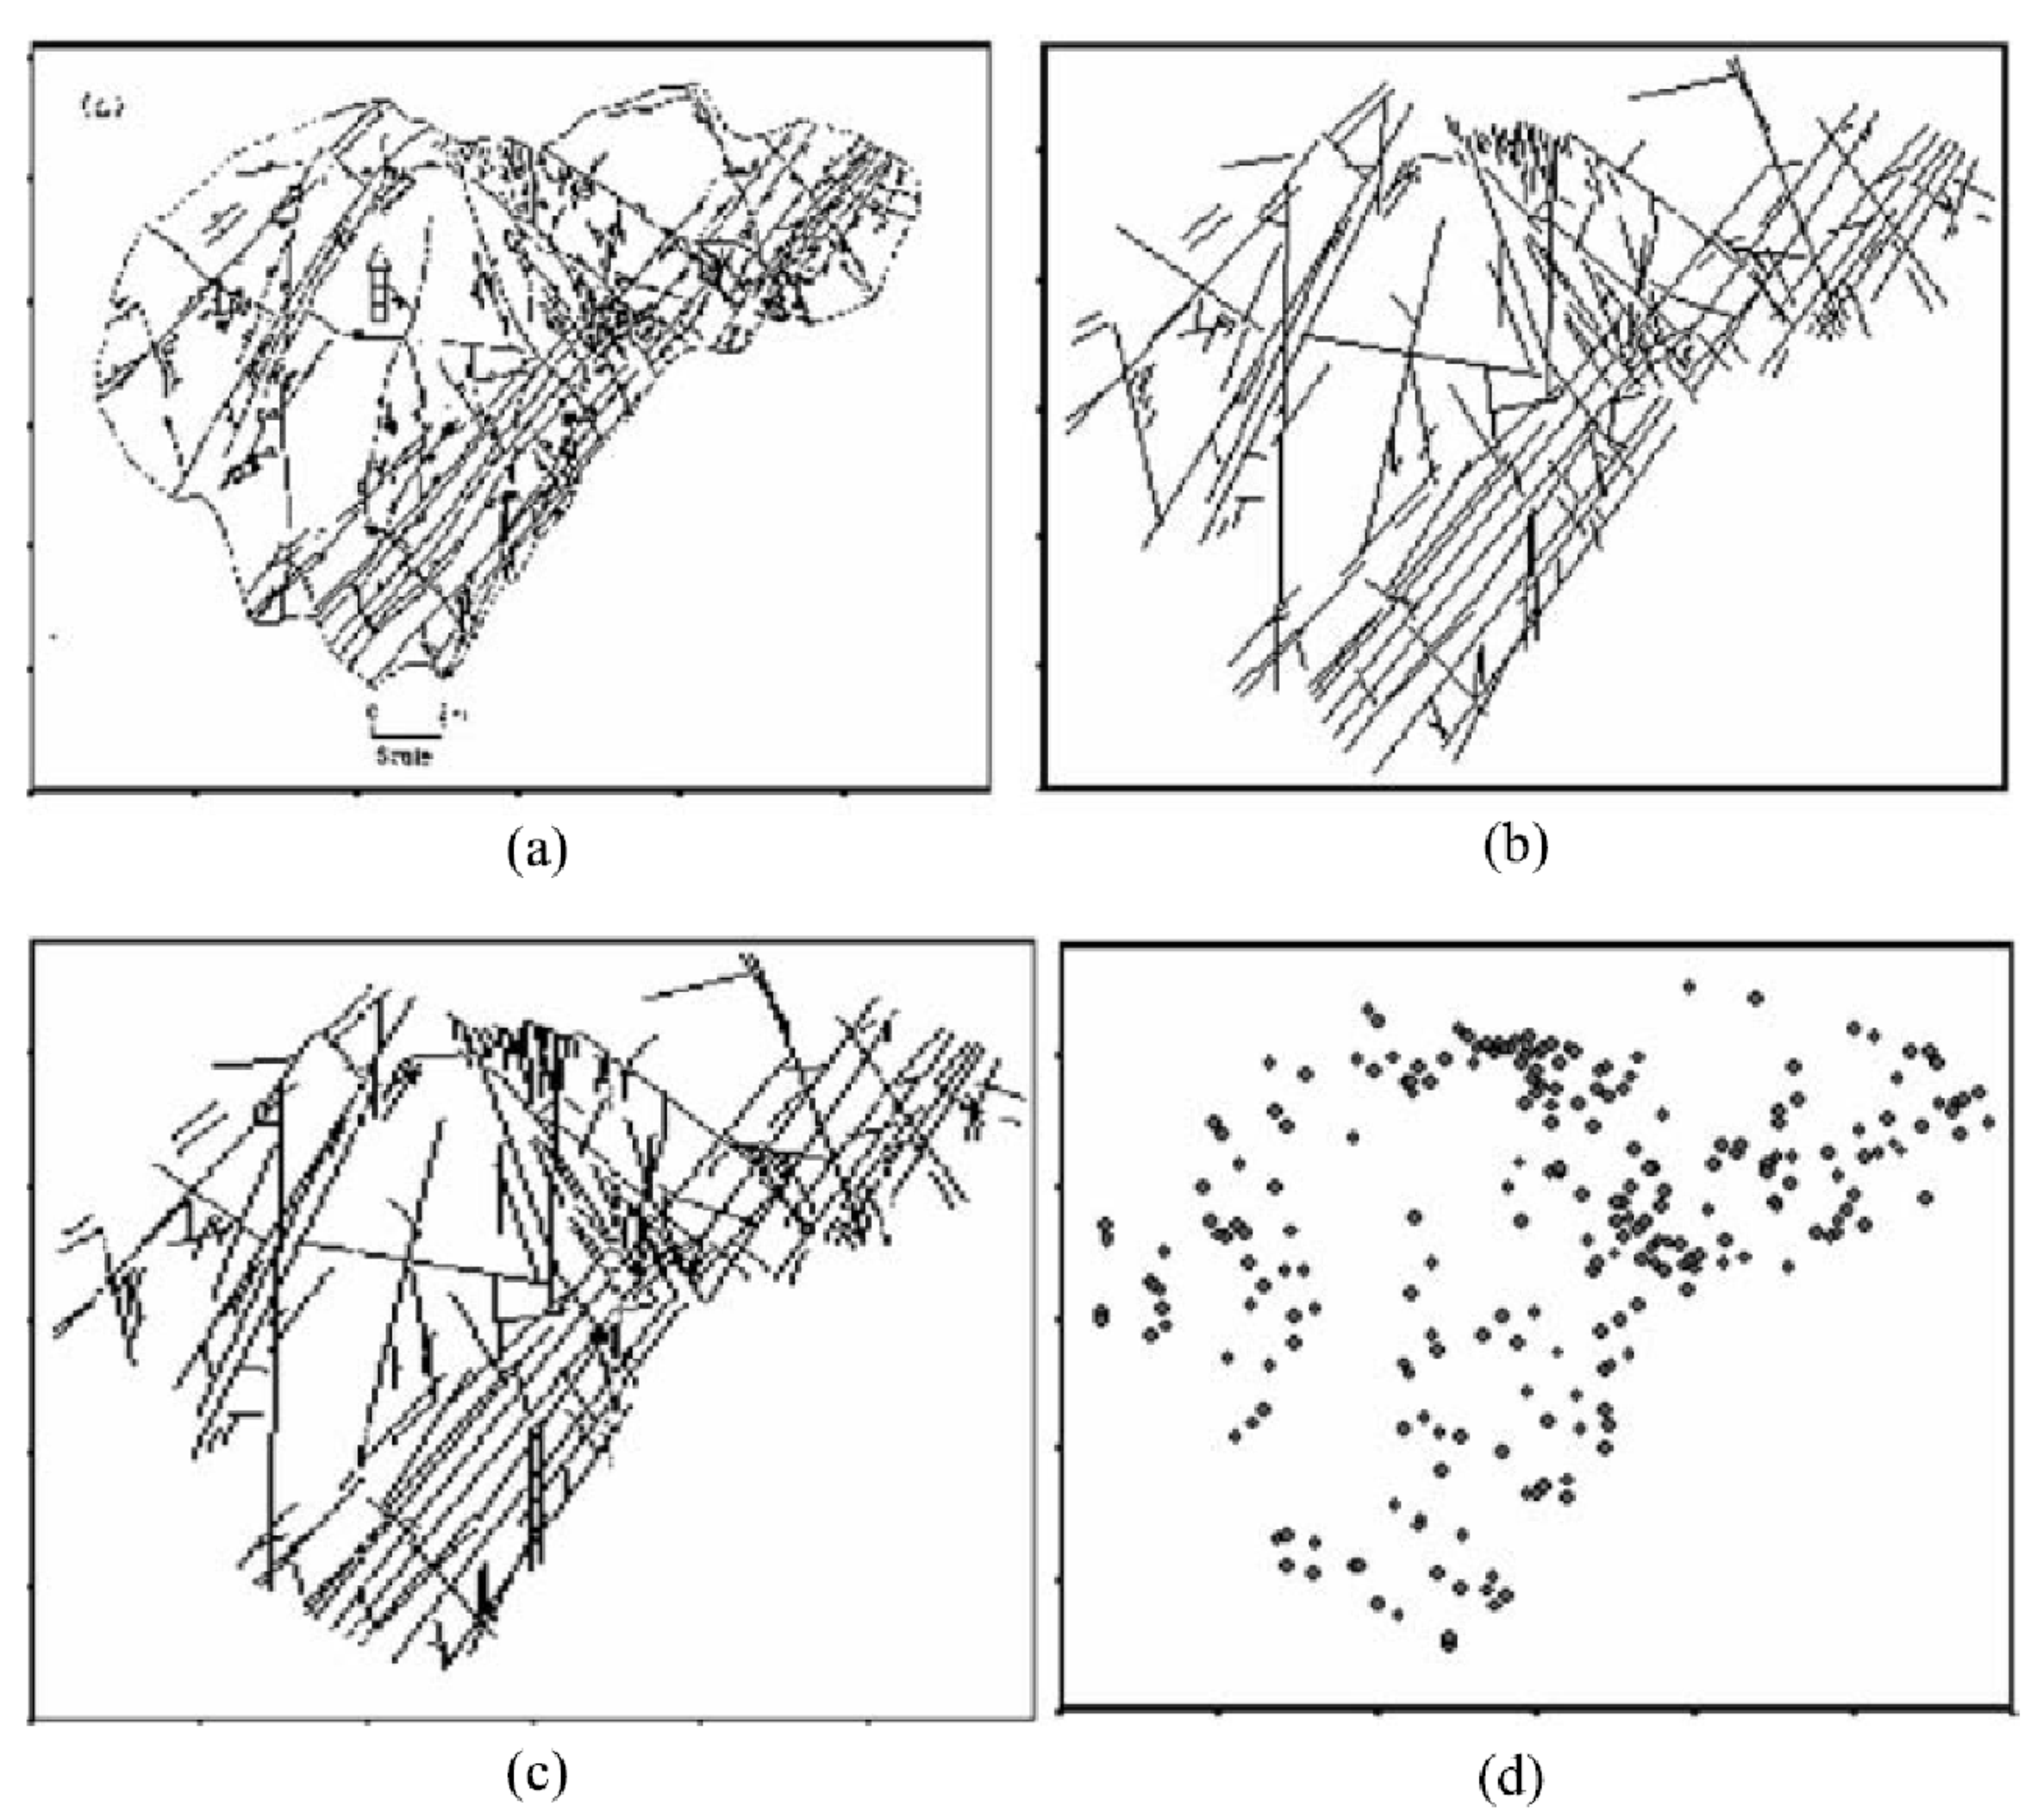
\includegraphics[width=0.8\textwidth]{fraxByIndicatorSim}
	\caption{a) fracturas; b) fracturas digitalizadas; c) Fracturas pixeladas; d) centroides de fracturas.}
	\label{f:fraxByIndicatorSim}
\end{figure}

La funci\'on indicador para la \autoref{f:fraxByIndicatorSim}-c) se define como

\begin{equation}
    \mathbbm{1}_{F}(x)=
\begin{cases}
	1,	& \text{si $x \in F$;}\\
	0,	& \text{en otro caso.}
\end{cases}
\label{e:indicatorFunc}
\end{equation}

\noindent
donde $F$ representa un conjunto, en este caso, el conjunto aleatorio de las fracturas "pixeladas". Por lo tanto, la simulaci\'on (no condicionada) puede ser realizada con el m\'etodo Gaussiano truncado, el cual a su vez utiliza variogramas. Los resultados de la modelaci\'on con este m\'etodo se muestran en la \autoref{f:fraxByIndicatorSimVario}.

\begin{figure}[H] 
	\centering
	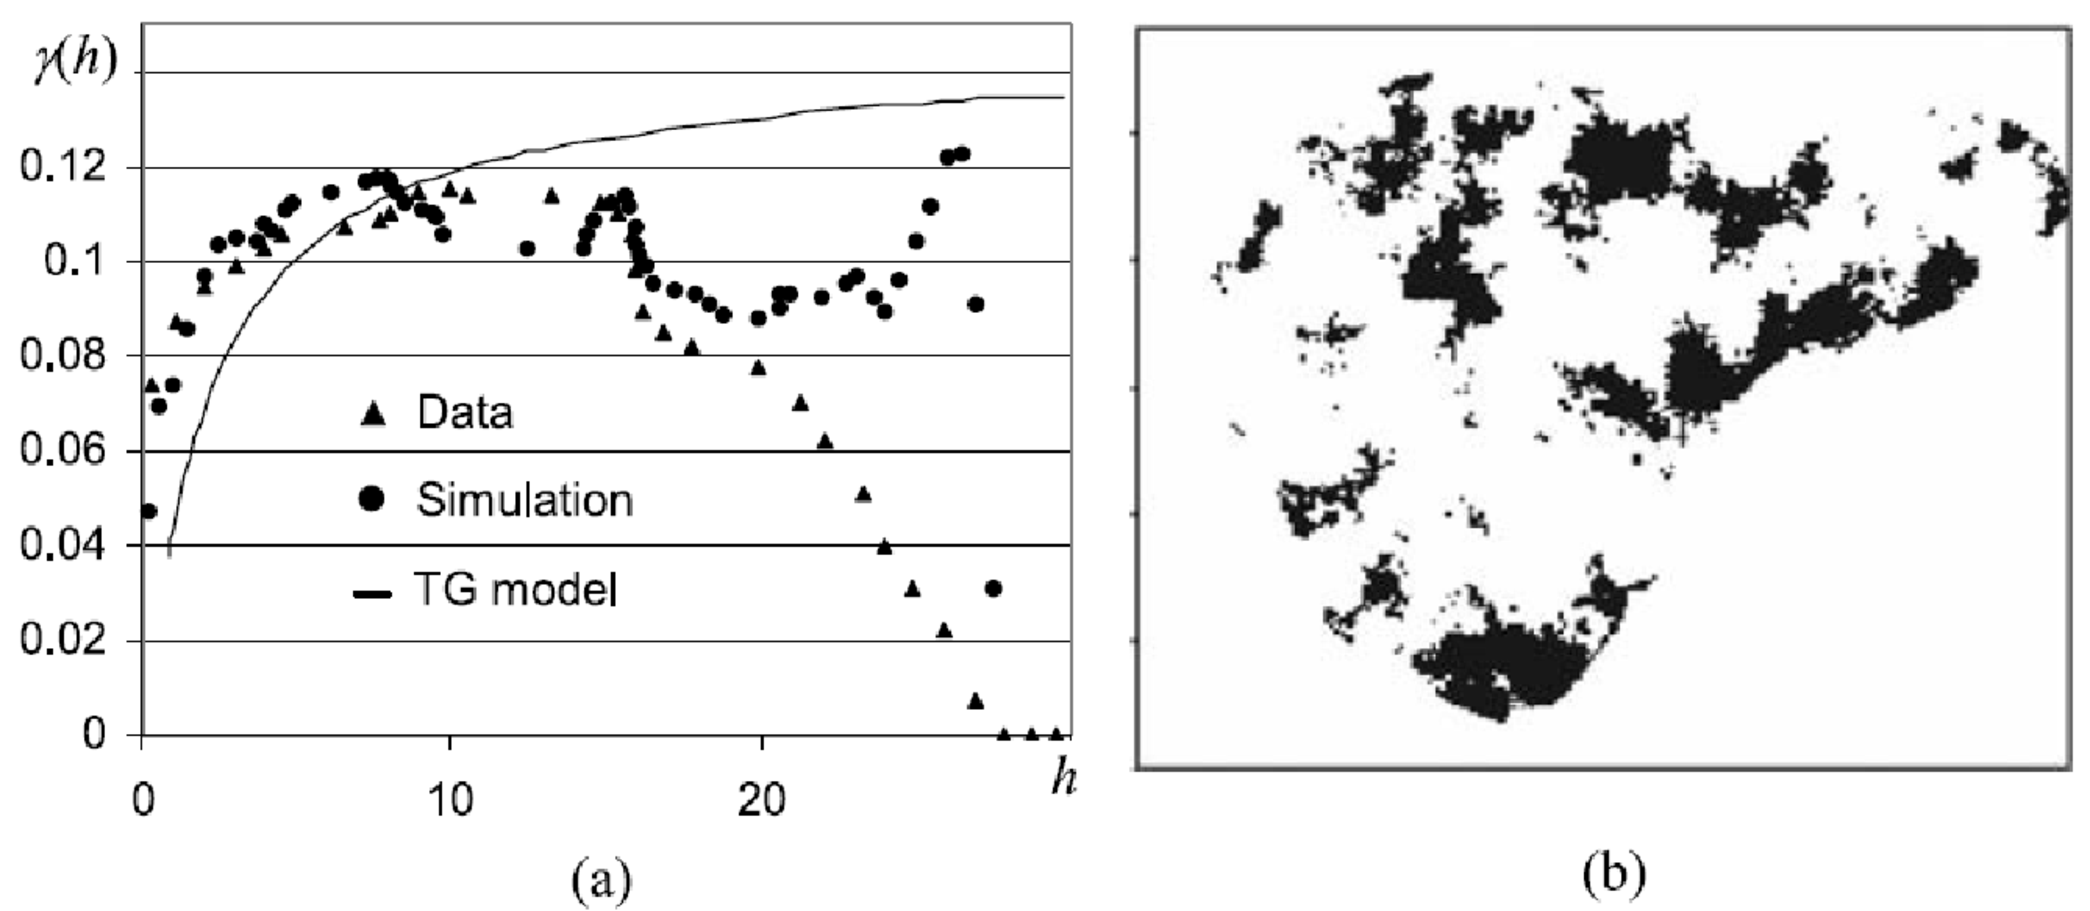
\includegraphics[width=0.8\textwidth, keepaspectratio = TRUE]{fraxByIndicatorSimVario}
        \caption{a) Variograma; b) Simulaci\'on. Modificada de la Fig. 2 de \citet{dowd_comparison_2007}}.
	\label{f:fraxByIndicatorSimVario}
\end{figure}

Aunque el modelo de variograma es reproducido razonablemente bien, la imagen simulada difiere considerablemente de la imagen original. Este ejemplo muestra que reproducir el primer orden y \'ordenes superiores de un campo aleatorio no necesariamente reproduce un proceso aleatorio.


\subsection{Modelo con geoestad\'istica multi-punto}

Utilizando el contexto de la geoestad\'istica convencional, el uso de s\'olo el primer y segundo momento es claramente insuficiente para simular las complejas estructuras de una red de fracturas. Utilizando las estad\'isticas de orden superior deber\'ia mejorar la simulaci\'on, aunque la reconstrucci\'on de todas las propiedades estoc\'asticas del campo aleatorio no se puede garantizar. La inferencia de orden superior en modelos estad\'isticos espaciales es dif\'icil, ya que se basan en las configuraciones espaciales en lugar de las distancias por pares y orientaciones simples usados en las formas tradicionales de la geoestad\'istica. Un enfoque consiste en utilizar la probabilidad condicional para una configuraci\'on particular para inferir experimentalmente el modelo espacial para describir el campo aleatorio.

Para una variable indicador, la probabilidad condicional es equivalente a la esperanza condicional de la configuraci\'on. La probabilidad condicional de que $\mathbbm{1}=1$, dado $n$ eventos $\mathbbm{1}(x) = 0$ \'o $1$ para $i = 1, \ldots, n$ se puede expresar como la suma de  t\'erminos de la siguiente manera:

\begin{equation}
	Prob
	\left\{
		\mathbbm{1} (x) = \mathbbm{1}(x_i), \qquad i = \{1,\ldots,n\}
		\\
		= \lambda_0 +
		\sum_{i=1}^n \lambda_i^{(1)} \mathbbm{1}(x_i) +
		\sum_{i=1}^n \sum_{j > i}^n \lambda_{ij}^{(2)}
		\mathbbm{1}(x_i) \mathbbm{1}(x_j) + \cdots
	\right\}
	\label{e:multiplePointG}
\end{equation}
	 	
Donde $\lambda_{\dots}^{()}$ son los $2^n+1$ coeficientes obtenidos por un sistema de Kriging simples extendidos. Los primeros $n+1$ t\'erminos se pueden resolver por Kriging (geoestad\'istica a dos puntos) y los otros t\'erminos describen el enfoque multi-punto de orden 3 al $n$.

Cuando se ha inferido la probabilidad condicional de la \autoref{e:multiplePointG}, $\mathbbm{1}(x)$ puede ser simulada mediante muestro Monte Carlo. Generalmente, la inferencia se basa en realizaciones de la variable aleatoria, a las cuales se les conoce como im\'agenes de entrenamiento. Estas im\'agenes de entrenamiento pueden ser datos o postulados en base a la experiencia. La simulaci\'on secuencial de $\mathbbm{1}(x)$ depende del n\'umero $n$ de datos indicadores, $\mathbbm{1}(x_i)$, m\'as cercanos a cada nodo $x$.

En la \autoref{f:fraxByMultiPoint} se muestran los resultados para diferentes valores de $n$. Estas simulaciones muestran la importancia de este  par\'ametro en la estad\'istica multi-punto. La selecci\'on de $n$ depende lo complejo de las estructuras a simular. En el ejemplo que aqu\'i se muestra se puede concluir que valores $n \le 12$ son inadecuados para describir el sistema de fracturas en cuesti\'on.

\begin{figure} 
	\centering
	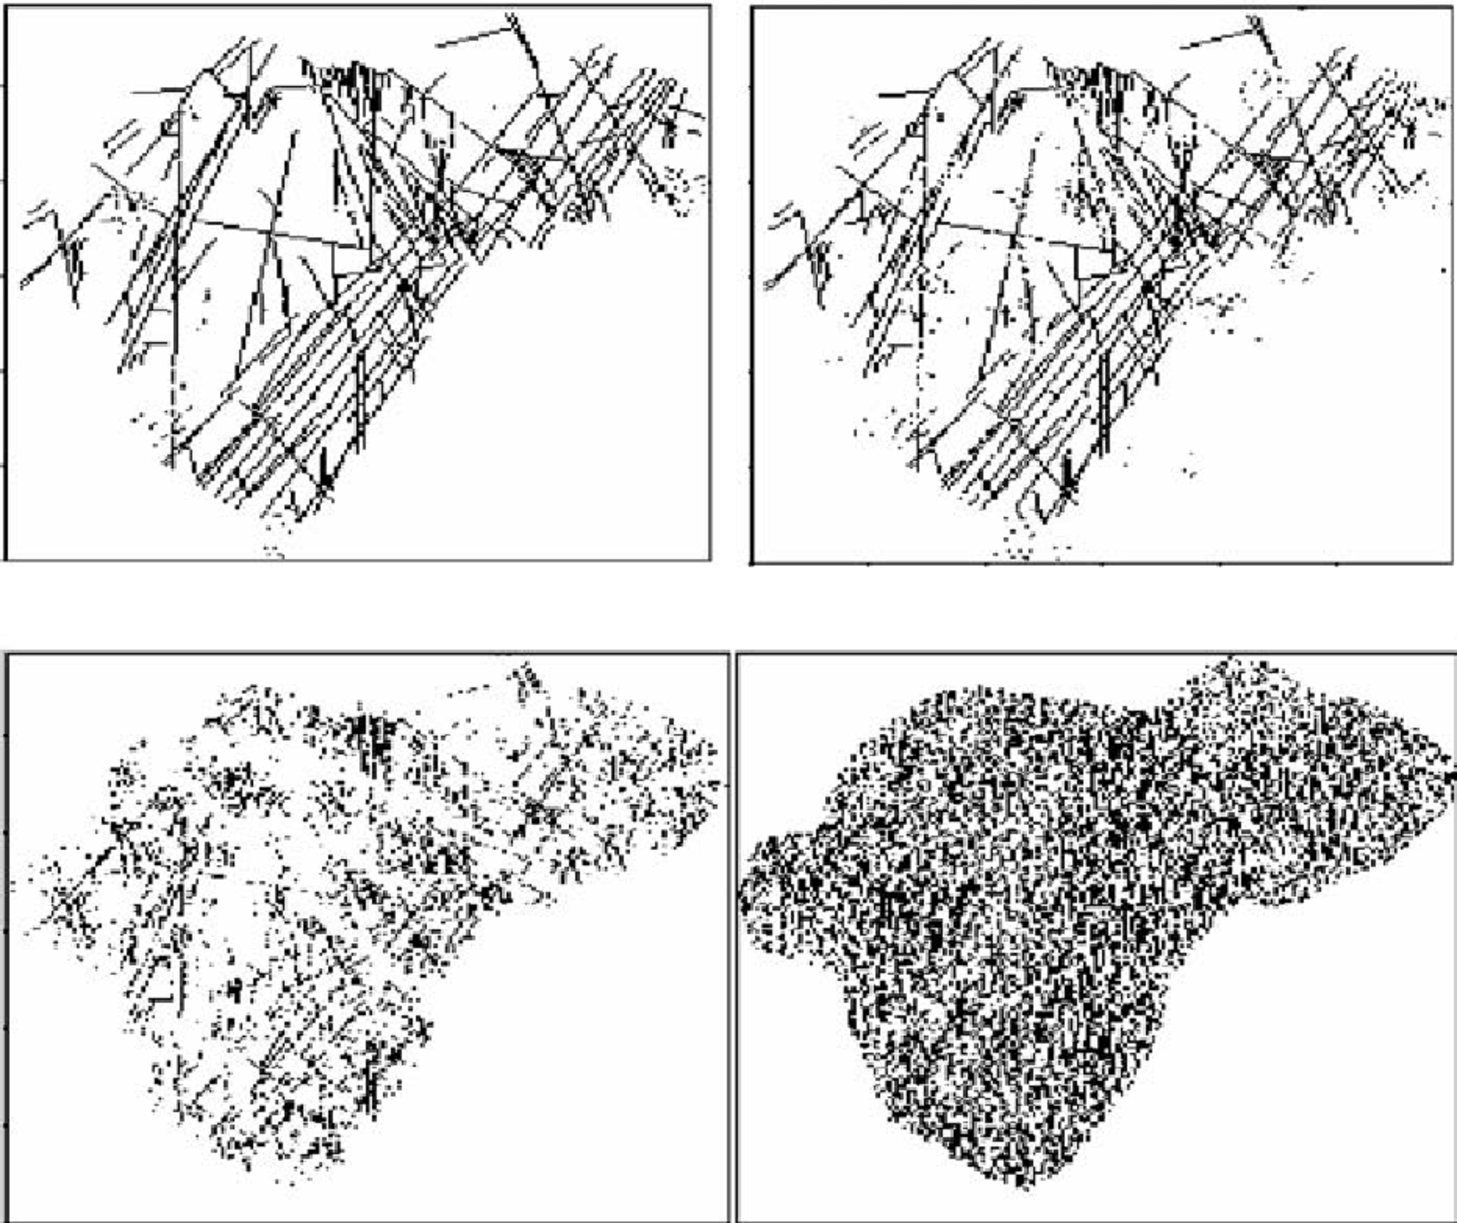
\includegraphics[width=0.8\textwidth, keepaspectratio = TRUE]{fraxByMultiPoint}
	\caption{Simulaciones basadas en la geoestad\'istica multi-punto.}
	\label{f:fraxByMultiPoint}
\end{figure}


\begin{table}
	\centering
\begin{tabular}{|l|c|c|}
\hline
$n$ & Pixeles negros (\%) & Posici\'on en la \autoref{f:fraxByMultiPoint} \\
\hline
\hline
20 & 19.63 & Superior izquierda\\ \hline
16 & 19.26 & Superior derecha\\ \hline
12 & 20.88 & Inferior izquierda\\ \hline  
8  & 43.97 & Inferior derecha\\ \hline
\end{tabular}
\caption{Valores de porcentajes de pixeles negros para los resultados en la \autoref{f:fraxByMultiPoint}.}
\end{table}

\subsection{Modelos booleanos}

Debido a la complejidad de las fracturas y m\'as a\'un de los sistemas de fracturas, no es viable modelarlas con demasiada precisi\'on. Por ejemplo, el simple hecho de intentar modelar las caras de las fracturas es computacionalmente lento. Si el objetivo buscado es la simulaci\'on de flujo, este \'ultimo puede tomar mucho m\'as tiempo si se considera la rugosidad de la fractura. En muchos de los casos, la rugosidad de estas superficies puede ser auto-af\'in, es decir tener propiedades fractales \citep[ch. 4]{adler_fractures_1999}.

Cuando se desea modelar un sistema de fracturas en alg\'un yacimiento, el enfoque del p\'arrafo anterior se torna imposible de implementar. Un enfoque m\'as viable es simplificar la geometr\'ia de las fracturas. Por ejemplo, se puede suponer que las caras son planos (\autoref{f:parallelPlates}), modelo conocido como de placas paralelas \citep{dietrich_flow_2005}.

\begin{figure}[H]
	\centering
	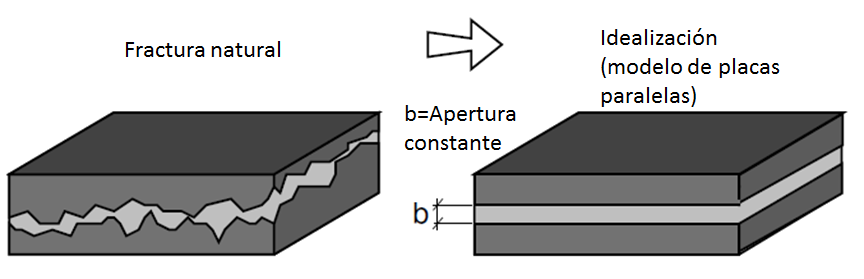
\includegraphics[width=0.7\textwidth]{parallelPlates}
	\caption{Modelado de una fractura. Izquierda: fractura real; derecha: su modelo de placas paralelas (Modificada de la Fig. 2.11 de \citeauthor{dietrich_flow_2005}, \citeyear{dietrich_flow_2005}).}
	\label{f:parallelPlates}
\end{figure}

Con el enfoque de \cite{dietrich_flow_2005}, se supone que las fracturas son discretas y simplificadas. Los modelos m\'as usuales para representar sistemas de fracturas en medios porosos en general y en particular en la modelaci\'on de Yacimientos Naturalmente Fracturados (YNF) son los modelos de Redes de Fracturas Discretas (DFN). Este tipo de modelos nos proporcionan el n\'umero de fracturas en determinado volumen con longitudes y orientaciones dadas. Estos modelos consideran a una fractura como un ente geom\'etrico simplificado, usualmente segmentos rectil\'ineos, paralelogramos y elipses en 2D, y pol\'igonos, paralelep\'ipedos y elipsoides en 3D. Por lo que una fractura discreta puede ser caracterizada por su longitud, apertura, orientaci\'on, etc. 

El m\'etodo estoc\'astico de simulaci\'on de fracturas discretas est\'a basado en el modelo booleano, el cual a su vez se construye a partir de procesos puntuales de Poisson que generan los centros geom\'etricos de los objetos que representan a las fracturas. Aqu\'i por objeto se est\'a considerando a los entes geom\'etricos que representan a las fracturas. Los objetos no son determin\'isticos, son aleatorios, es decir \'estos son generados estoc\'asticamente, por lo que sus caracter\'isticas geom\'etricas est\'an dadas por funciones de distribuci\'on de probabilidad.

La aplicaci\'on de los modelos booleanos no solamente se restringe a la generaci\'on de las redes de fracturas si no tambi\'en dentro de la teor\'ia de percolaci\'on continua. Esta teor\'ia cuantifica la probabilidad de que las fracturas generadas est\'en conectados y que ellas formen una trayectoria entre dos ubicaciones especiales dadas. En la tesis de \citet{ayala-garcia_estimacion_2014} se muestran algunos casos de percolaci\'on utilizando redes de fracturas similares, mas no iguales, a las que se trabajaron en esta tesis.

Dado que \'este es el enfoque computacionalmente m\'as viable para la modelaci\'on de fracturas en un yacimiento, es el que se adopt\'o en este trabado doctoral. En el siguiente cap\'itulo se explica m\'as la teor\'ia de los modelos booleanos. Por lo pronto diremos que la idea intuitiva es la de objetos simplificados aleatoriamente colocados en el espacio. La palabra aleatoria se utiliza en un sentido probabil\'istico y no significa que est\'en uniformemente distribuidos.

